\documentclass{article}
\usepackage[utf8]{inputenc}
\usepackage{amssymb}
\usepackage{graphicx}


\title{IFT3335-TP1-Rapport}
\author{Wenhao Xu, 20150702\\
Mingze Li, \\
Yu Deng, 20151659}

\date{}

\begin{document}

\maketitle

\section*{Tâche 1 et Tâche 2}\\
On test dans le programme \textbf{sudoku\_final.py}, avec les appels suivants:\\\\
\textbf{solve\_all(from\_file("100sudoku.txt"),"easy", None)}, ce qui est un appel du programme de Norvig original\\
\textbf{solve\_all\_pur\_profondeur(from\_file("100sudoku.txt"),"easy", None)}, ce qui est un appel à une recherche pure en profondeur d’abord sans aucune heuristique.\\
Voici est le résultat:\\
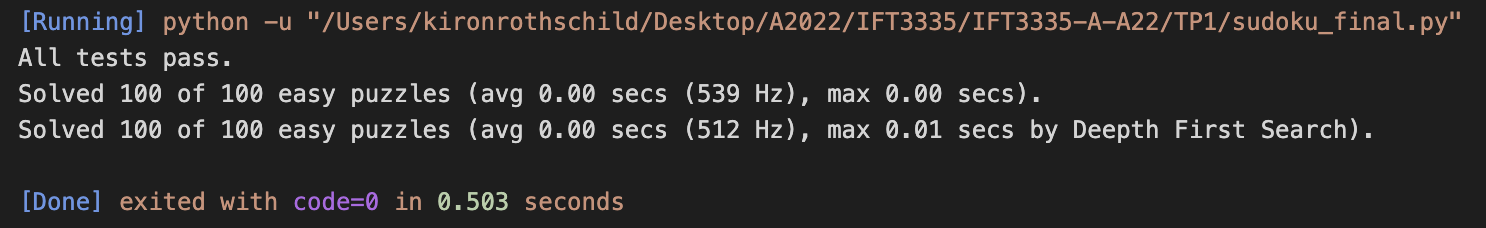
\includegraphics[width=1\textwidth]{t2.png}\\
Après plusieurs exécutions différentes du programme, les performances de la recherche non heuristique DFS se dégradent à chaque fois par rapport à la recherche initiale, même si les valeurs ne sont pas exactement les mêmes à chaque fois.\\
Nous pouvons en déduire que pour le deuxième code(la recherche non heuristique DFS), nous avons besoin d'un peu plus de temps, même si la différence n'est pas très grande, mais cela montre aussi l'importance de l'heuristique.

\section*{Tâche 3}\\
Dans la tâche 3, on a implémenté avec succès les heuristiques Naked Pairs/Triples \& Hidden Pairs/Triples\\
Avec l'appel \textbf{solve\_all\_heuristique(from\_file("100sudoku.txt"),"easy", None)}, on a obtenu le résultat:\\
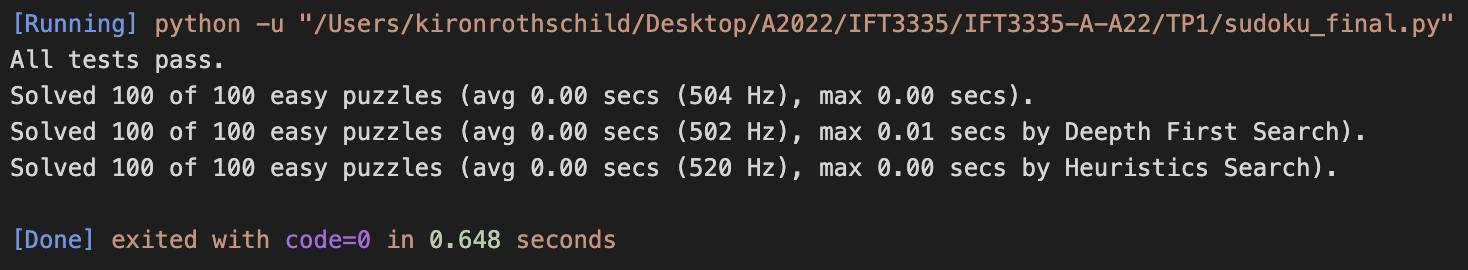
\includegraphics[width=1\textwidth]{t3.png}\\
On peut voir que, bien que l'ampleur soit faible, les performances de l'algorithme se sont quelque peu améliorées par rapport à l'algorithme initial.\\
On peut voir que, bien que l'ampleur soit faible, les performances de l'algorithme se sont quelque peu améliorées par rapport à l'algorithme initial. Cette amélioration modeste peut être due au fait que le cas Naked Pairs/Triples \& Hidden Pairs/Triples n'est pas toujours satisfait, et que si l'heuristique utilisée est d'une grande complexité et n'est pas optimisée pour les performances (le cas où la condition n'est pas satisfaite). Il y a également un certain degré de perte de performance.


\section*{Tâche 4 et Tâche 5}\\
Voici le résultat de l'appel\\
\textbf{solve\_all\_hill\_climbing(from\_file("100sudoku.txt"),"easy", None)}:\\
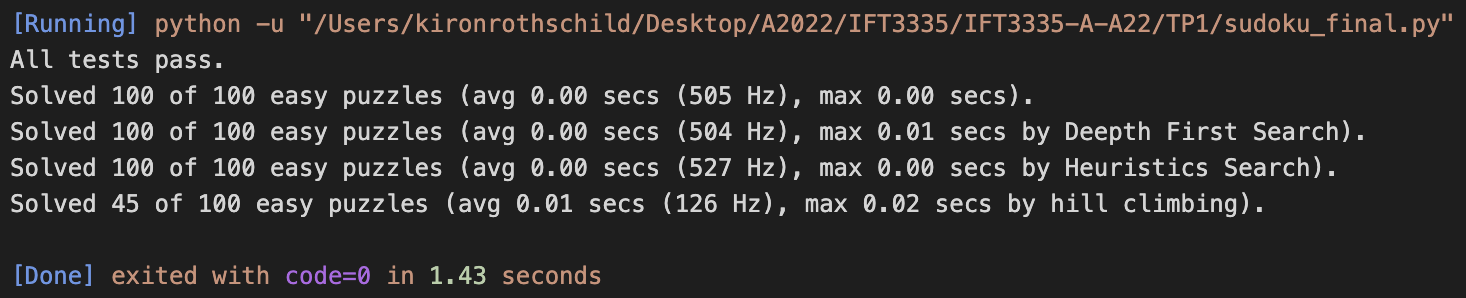
\includegraphics[width=1\textwidth]{t4.png}\\
Il est facile de voir que pour l'algorithme Hill-Climbing, il y a une baisse significative du taux de réussite et des performances. Cela est dû aux limites de l'algorithme Hill-Climbing, qui produit une solution localement optimale mais pas nécessairement une solution globalement optimale. Il est donc possible que nous n'obtenions pas de réponse au Sudoku.\\
Il est facile de voir que pour l'algorithme Hill-Climbing, il y a une baisse significative du taux de réussite et des performances. Cela est dû aux limites de l'algorithme Hill-Climbing, qui produit une solution localement optimale mais pas nécessairement une solution globalement optimale. Il est donc possible que nous n'obtenions pas de réponse au Sudoku.
Une optimisation de l'algorithme Hill-Climbing est l'algorithme Simulated-Annealing. Cependant, étant donné que l'algorithme Simulated-Annealing est très complexe, qu'il entraîne toujours une perte de performance significative (par rapport à l'algorithme initial) et qu'il nécessite l'utilisation de l'algorithme Hill-Climbing, nous n'avons finalement pas implémenté l'algorithme Simulated-Annealing.


\end{document}
